%!TEX root = Main.tex
\section{Implementation}
The following chapter seeks to explain the implementation of the mini project.\\

\subsection{Overall Design}
Image and explanation of the overall system and blocks\\
\begin{figure}[H]
	\centering
	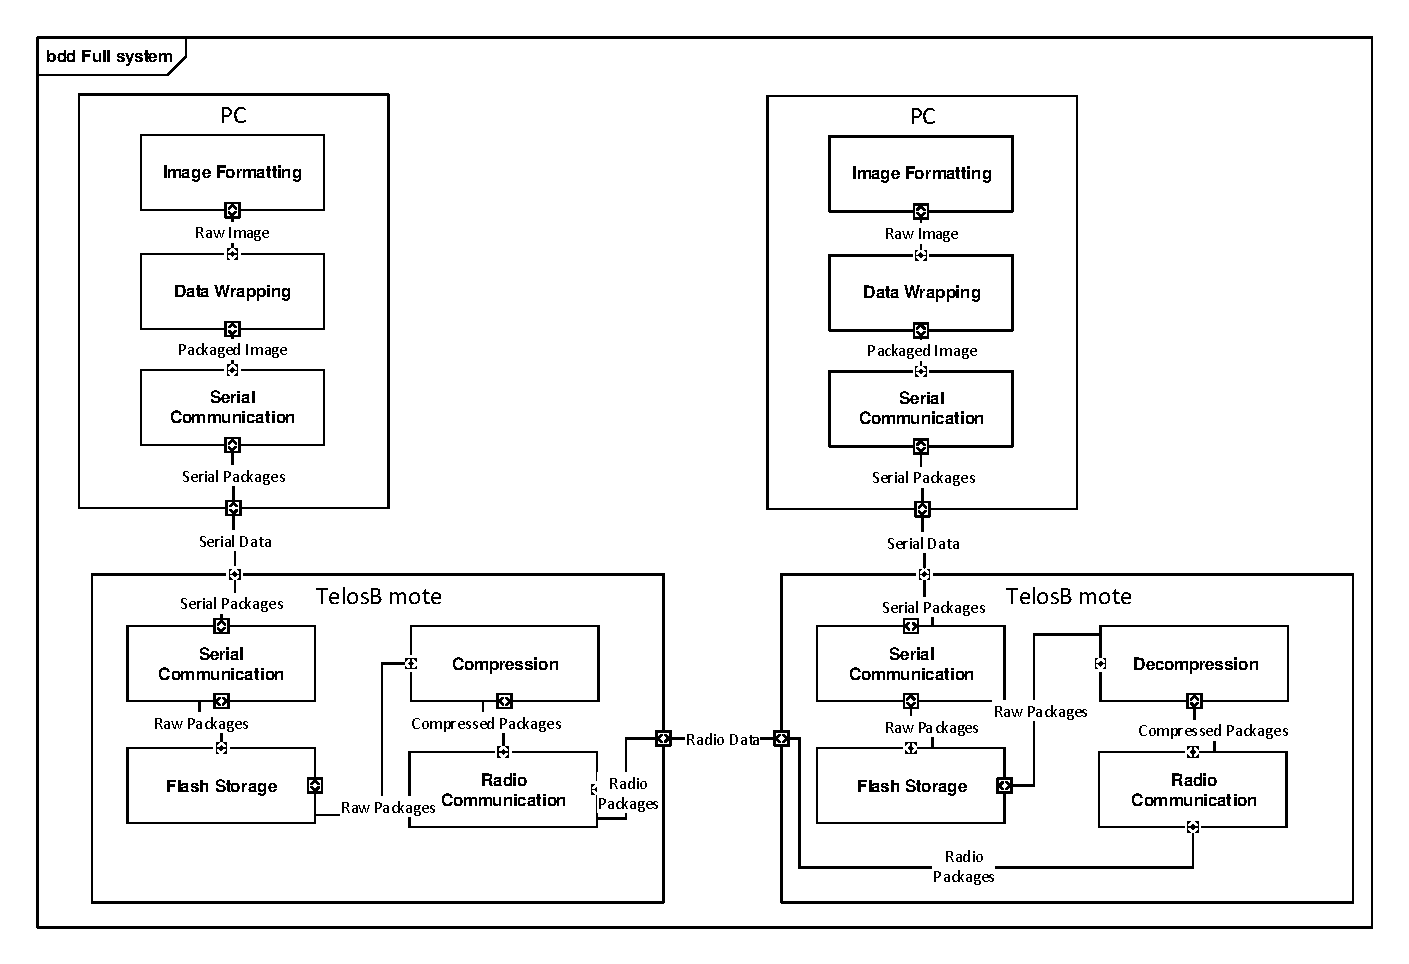
\includegraphics[width=1\textwidth]{FullSystem}
	\caption{Full System Diagram.}
	\label{FullSystem}
\end{figure}

\subsection{Serial communication}
The serial communication is responsible for the transfer of the image to and from the TelosB. A header file is available to both the PC software and the TelosB program. It contains a series of defines that are used for the communication messages. The defines can be found in table \ref{definetable}.
\begin{table}[H]
    \begin{tabular}{|l|l|l|}
    \hline
    Name                  & Val & Description                                               \\ \hline
    TRANSFER\_TO\_TELOS   & 1     & Used to tell the TelosB to prepare to receive the image. \\ \hline
    TRANSFER\_OK          & 2     & Used to tell the PC that the transfer was ok.             \\ \hline
    TRANSFER\_FAIL        & 3     & Used to tell the PC that the transfer failed.             \\ \hline
    TRANSFER\_READY       & 4     & Used to tell the PC that the transfer can be initiated.   \\ \hline
    TRANSFER\_FROM\_TELOS & 5     & Used to tell the TelosB to transfer the image to the PC.  \\ \hline
    TRANSFER\_DONE        & 6     & Used to tell the PC that the image transfer is done.      \\ \hline
    \end{tabular}
    \caption{Defines for serial communication.}
    \label{definetable}
\end{table}
\begin{figure}[H]
	\centering
	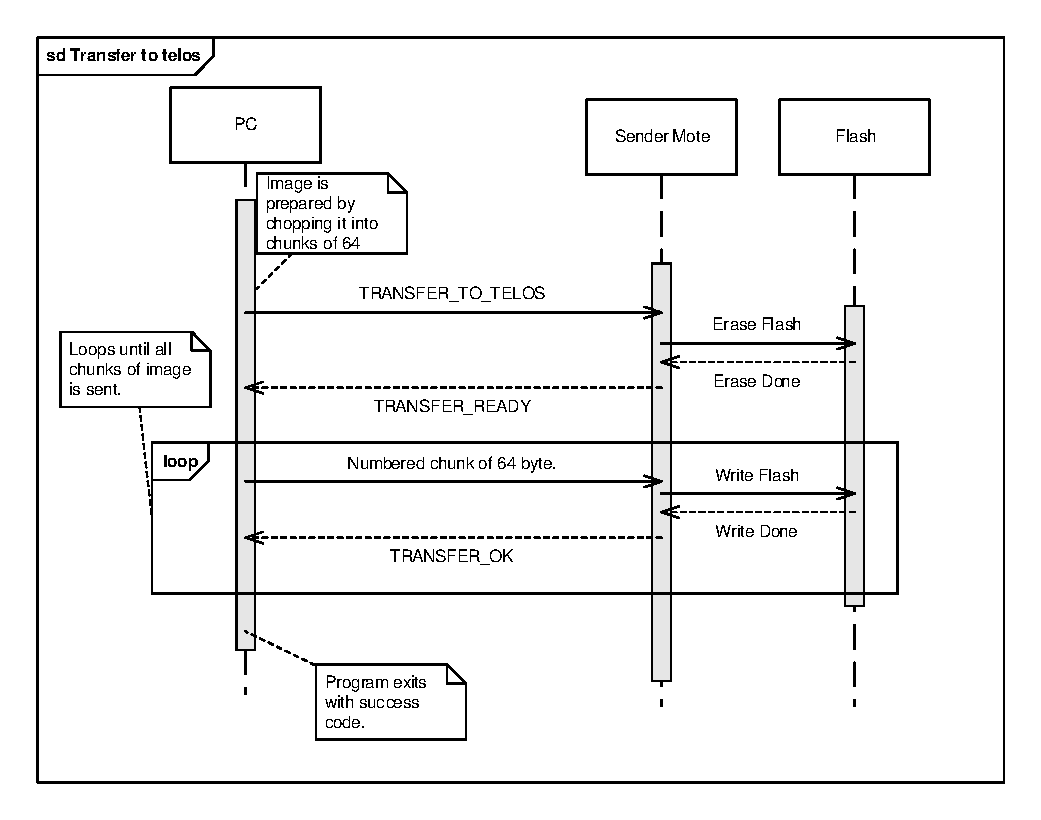
\includegraphics[width=0.8\textwidth]{PCtoTelosb}
	\caption{Transfer to TelosB sequence diagram.}
	\label{transfertotelos}
\end{figure}

\begin{figure}[H]
	\centering
	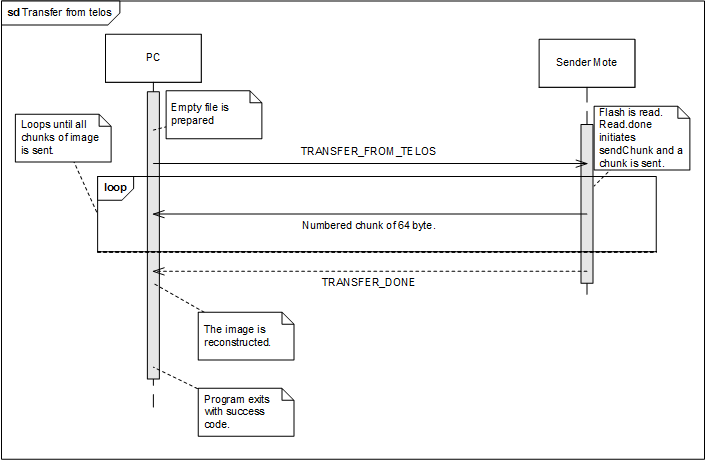
\includegraphics[width=0.8\textwidth]{PCfromTelosb}
	\caption{Transfer from TelosB sequence diagram.}
	\label{transferfromtelos}
\end{figure}

\subsection{Radio Block}

\subsection{Compression block}
The compression blocks have a common interface: 

\begin{itemize}
    \item \texttt{uint16\_t Compress(uint8\_t* in, uint8\_t* out)}
    \item \texttt{void Decompress(uint8\_t *in, uint8\_t *out)}
\end{itemize}

This interface allows the different implementation to be accessed with the same code -- only specifying the desired block.

The \texttt{Compress(...)} method will take 1024 bytes in its first parameter, and return the compressed data in its second parameter, and return the size of the compression as return output.

The \texttt{Decompress(...)} method will, too, take the input as the first parameter and output as second parameter. 
The \texttt{Decompress(...)} method already knows how big the input is, and the output will always 
